\begin{Omitir}
Un método menos drástico es considerar modelos gaussianos. En estos, el sistema se considera completamente especificado mediante correlaciones de pares de modos bosónicos.La dinámica exacta puede ser estudiada a a partir de la ecuación de Heinsenberg con un Hamiltoniano que incluya los términos libres de interacción junto a estas interacciones de forma tal que se respeten las propiedades del sistema.
\end{Omitir}

\begin{Omitir}
En el presente trabajo, se analizará la dinámica gaussiana  de sistemas cuánticos abiertos y la dinámica de sistemas cuánticos cerrados mediante una aproximación de estados instantáneos Max-Ent. Además, se utilizó la librería QuTip del lenguaje Python para simular la dinámica de dichos sistemas cuánticos estudiados y estudiar la correspondencia de los resultados analíticos con los resultados numéricos. 
\end{Omitir}

\begin{Omitir}

\footnote{Formalmente, tendremos una función medible \cite{Portesi-ECI34} $\mathcal{X}: (\Omega, \mathcal{A}, P) \rightarrow (\mathds{R},\mathcal{B}(\mathds{R}, P_\mathcal{X})$, donde $(\Omega,\mathcal{A})$ es un espacio medible formado por un espacio muestral $\Omega$ y una colección $\mathcal{A}$ de subconjuntos de $\Omega$ el cual dispone de una función de medida de probabilidad $P : \mathcal{A} \rightarrow \mathbb{R}_{+}$ la cual tiene la condición $P(\Omega) = 1$. Dicha medida $P_\mathcal{X}$ sobre el Boreliano $\mathcal{B}(\mathbb{R})$ se llama la \textit{distribución de probabilidad} de $\mathcal{X}$. }

\end{Omitir}

\begin{Omitir}
{\color{red}Como cualquier observable asociado a una de estas partes es compatible con cualquier observable asociado a otra de esas partes, el espacio de estados del sistema completo queda representado como el producto tensorial de los espacios de estados de cada subsistema. Esto motiva el siguiente:}{\color{blue}  Hacemos uso del producto tensorial para enunciar el siguiente postulado}
\end{Omitir}

\begin{Omitir}
Los postulados de la mecánica cuántica \ref{Post1}, \ref{Post time evolution}, \ref{Post measurement}, \ref{Post separability} proveen de un marco de trabajo para la descripción de un sistema físico. Sin embargo, como todo modelo físico, aún se necesita conocer información acerca del sistema e introducir hipótesis sobre el mismo. Por otro lado, estos postulados no son inmediatamente adecuados para la descripción de la dinámica de sistemas abiertos.
\end{Omitir}
\begin{Omitir}
%\subsection{Consecuencias de los postulados }
 
\notaFTBP{Capaz que esta sección simplemente la puedo eliminar porque no es que realmente la usé en el tdd directamente ni hice mención de ella.}
 
Los postulados anteriormente enunciados tienen importantes consecuencias, algunas de las cuales son enunciadas en la presente sección. 
  
\begin{enumerate}
 \item  Una \textbf{medida Proyectiva} es una medida definida en términos de proyectores ortogonales $\Pi_{m}$. Si todos los $\Pi_m$ son de rango 1, la medida será \textit{completa}. En tal caso, el estado del sistema luego de la medida queda completamente determinado \cite{Nielsen.00}. 
 
\item Dados dos estados, se los podrá distinguir mediante una medida proyectiva. Esto será posible únicamente si los estados son ortogonales. Una consecuencia de esto es el \textit{teorema de no-clonación}: dado un estado cuántico desconocido, sólo es posible " copiarlo" si se conoce la base en la que es diagonal \cite{Nielsen.00}.
 
\item La dimensión del espacio de Hilbert de un espacio compuesto crece exponencialmente con el número de componentes.
 
\item Dado un conjunto de operadores de Kraus, existen infinitas elecciones de otros operadores de Kraus que producen una evolución equivalente. 
 
\item Toda evolución de la forma de \eqref{state evolution} puede obtenerse en términos de una evolución unitaria conjunta entre el sistema objetivo y un sistema auxiliar, seguida de la traza parcial sobre el sistema auxiliar. Esto es la dilatación de Stinespring \cite{Stinespring,KasparovabtSt.}
\end{enumerate}
\end{Omitir} 

\begin{Omitir}
footnote{En el formalismo de Cox \cite{KNUTH2005245}, la información de Shannon surge como la medida natural de la información mientras que la entropía de von Neumann aparece como la medida natural en el álgebra no Booleana de la mecánica cuántica \cite{holik2015natural}. En cierta forma, la teoría de la información cuántica es una versión \textit{no Kolmogoroviana} de la teoría de la información clásica \cite{e17117349}.}
\end{Omitir}

\begin{Omitir}
lo que es formalmente un Hamiltoniano de dos sistemas bosónicos no interactuantes. La solución a dicho Hamiltoniano ya es conocida. Ahora bien, cuál es el valor de expectación de dicho Hamiltoniano en términos de los valores de expectación de los operadores bosónicos originales; de los cuales obtenemos el número de partículas en cada subsistema. Obtendremos que

\begin{dmath}
    \lgg {\bf H}\rgg = \bigg(\Omega_1 |P_{11}|^2+\Omega_2 |P_{12}|^2\bigg)^2 \lgg {\bf a}^{\dagger} {\bf a} \rgg + \bigg(\Omega_1 |P_{21}|^2+\Omega_2 |P_{22}|^2\bigg)^2 \lgg {\bf b}^{\dagger} {\bf b} \rgg  \\
    + \bigg(\Omega_1 P_{21}^{*}P_{11}+\Omega_2 P_{22}^{*}P_{12}\bigg)^2 \lgg {\bf a}^{\dagger} {\bf b} \rgg + \bigg(\Omega_1 P_{12}^{*}P_{22}+\Omega_2 P_{11}^{*}P_{21}\bigg)^2 \lgg {\bf b}^{\dagger} {\bf a} \rgg. 
\end{dmath}

Notamos que $\lgg {\bf a}^{\dagger} {\bf a} \rgg = n_A$, el número de ocupación bosónico del sistema $A$ y análogamente con $\lgg {\bf b}^{\dagger} {\bf b} \rgg = n_B$. Del cálculo anterior observamos que las correlaciones introducidas en el sistema como producto de la inclusión del término de interacción en el Hamiltoniano \eqref{model3.1_hamiltonian} cambian la temperatura efectiva del bosón aislado. 

%{\Huge \color{red} Esta parte estaría bien completarla: Primero viendo cómo construir el estado reducido usando que el estado es gaussiano, y luego mostrando la forma explícita del coeficiente que te queda. No es algo super largo, pero hace al manejo de estas expresiones que vamos a usar después. La parte de la reducción del estado global al estado local la podés sacar del borrador del paper, o del papar con Rossignoli y Canosa de 2013.}
\end{Omitir}

\begin{Omitir}
{\color{blue}(No va)
Podremos clasificar los sistemas cuánticos acorde a la posibilidad de interacciones con su entorno; los sistemas cerrados son aquellos que no interactúan con su entorno y se encuentra gobernada por la ecuación de Schrödinger\cite{HeinzPetruccione}\cite{Sch35} mientras que la dinámica de sistemas cuánticos abiertos son aquellos que interactúan con su entorno y se encuentra gobernada por la ecuación de Lindblad \cite{HeinzPetruccione}\cite{Lindblad1976}.}

En muchos sistemas, existen componentes bien definidas que interactúan entre sí de alguna forma. 


En el modelo de dos sistemas bosónicos acoplados, al estudiar la dinámica abierta a cortos plazos, hicimos uso del teorema de Picard, del Principio Max-Ent y usamos la traza parcial para poder eliminar las correlaciones existentes entre ambos sistemas. 

En esta sección buscaremos estudiar el comportamiento de las entropías relativas y de los valores de expectación de algunos operadores frente a diferentes rutinas numéricas.
\end{Omitir}



\begin{Omitir}
\begin{definition}

Un \textbf{proceso de Markov clásico} es un proceso estocástico general $\mathbf{X}(t)$ a tiempo discreto $\{X_n : n=0,1,2,\ldots\}$ con espacio de estados discreto $S$ que para cualquier entero $n\geq0$ y para cualesquiera $x_0,x_1,\ldots,x_{n+1} \in S$ satisface

\begin{equation}
    P[X_{n+1} = x_{n+1} |X_0 = x_0, X_1 = x_1, \ldots, X_n = x_n] = P[X_{n+1}=x_{n+1}|X_n = x_n],
    \label{Markov property}
\end{equation}

donde $P(A|B)$ es la probabilidad condicional de $A$ dado el evento $B$. A la ecuación anterior se le conoce como \textbf{propiedad de Markov}.
\end{definition}
\end{Omitir}



\subsection{Teorema espectral y operadores auto-adjuntos}

La base matemática de la teoría cuántica se halla en el teorema espectral y en la correspondencia entre observables físicos y operadores autoadjuntos. Esta relación se basa en el siguiente postulado

\begin{post}\textbf{Sobre el espacio de estados}
Sea un sistema físico aislado, existe un espacio vectorial complejo asociado, provisto de un producto interno, el cual es completo y separable \ie. un espacio de Hilbert denotado por $\mathbb{H}$. En este espacio se encuentran todos los \textbf{vectores de estado} que caracterizan el sistema. Diremos que $\mathbb{H}$ es el espacio de estados. 
\label{Post state space}
\end{post}

En mecánica cuántica, un estado de un sistema cerrado es descripto por un estado $\ket{\psi}$ el cual es un elemento de un espacio de Hilbert $\mathbb{H}$. Este espacio está provisto de un producto interno complejo. Sea $\bra{\phi}$ el elemento dual a $\ket{\phi}$, el cual pertenece al espacio dual $\mathds{H}^{*} \cong \mathds{H}$, luego el producto interno entre $\ket{\phi}$ y $\ket{\psi}$ se denota por $\bra{\phi} \ket {\psi}$. En consecuencia, la norma de un vector se define como 

\begin{equation}
    ||\psi|| = \sqrt{\bra{\psi} \ket {\psi}}.
\end{equation}

Sea $\mathbf{A} : \mathds{H} \rightarrow \mathds{H}$. Dicho operador se dice \textbf{acotado} si la \textbf{norma} de $\mathbb{A}$ 

\begin{equation}
    ||\mathbf{A}|| \doteq \sup_{\psi \in \mathds{H}-{0}} \frac{||\mathbf{A} \psi||}{||\psi||}
\end{equation}
es finita. El espacio de operadores acotados sobre $\mathds{H}$ forma un espacio de Banach, denotado por $\mathcal{B}(\mathds{H})$ frente a la operación de norma (de un operador) pues $\forall\mathbf{A}, \mathbf{B} \in \mathcal{B}(\mathbb{H}), || \mathbf{A}\mathbf{B} || \leq || \mathbf{A}|| ||\mathbf{B}||$.

Para todo operador $\mathbf{A} \in \mathcal{B}(\mathbb{H})$, existe un único operador $\mathbf{A}^{*}$, el \textbf{operador adjunto}, que cumple

\begin{equation}
    \lgg \phi, \mathbf{A} | \psi \rgg = \lgg \mathbf{A}^{*} \phi| \psi\rgg 
\end{equation}
para todo $\phi, \psi \in \mathbb{H}$. Un operador $\mathbf{A} \in \mathcal{B}(\mathbb{H}) $ se llama \textbf{autoadjunto} si $\mathbf{A}^{*} = \mathbf{A}$.

Para operadores no acotados, esto es operadores con norma no finita, cambian las condiciones en las cuales un operador es autoadjunto. Un operador no acotado, $\mathbf{C}$ se dice autoadjunto si

\begin{itemize}
    \item $Dom (\mathbf{C}) = Dom (\mathbf{C}^{*})$ 
    \item y $\mathbf{C}^{*}\phi = \mathbf{C}\phi$, para todo $\phi \in Dom (\mathbf{C}) $.
\end{itemize}

Finalmente, diremos que un operador no acotado $\mathbf{A}$ es una \textbf{extensión} de un operador no acotado $\mathbf{B}$ si $Dom(\mathbf{A}) \supset Dom(\mathbf{B})$.

Es posible demostrar el siguiente teorema \cite[p.~230]{HoracioI}
\begin{theorem}
Si el operador lineal $\mathbf{A}: \mathcal{S} \rightarrow \mathcal{S}$ es simétrico, continuo y admite una extensión autoadjunta en $\mathbb{H}$, entonces la extensión de $A$ a $\mathcal{S}^{*}$, $\mathbf{A}^{*}$, admite en ese espacio un sistema \textbf{ortogonal} y \textbf{completo} de distribuciones propias correspondientes a autovalores reales, que converge en el sentido de las distribuciones 
\label{Horacio teorema 7.1}
\end{theorem}

Mediante \ref{Horacio teorema 7.1} y usando que el espacio de Hilbert es separable, esto implica la existencia de un conjunto completo ortonormal $\{\phi_{\alpha}\}$, denso en $\mathcal{H}$, de vectores que cumplen 

\begin{equation}
    \bra{\phi_{\alpha}} \ket{\phi_{\beta}} = \delta_{\alpha \beta},
\end{equation}

de forma que todo estado $\ket{\psi}$ tiene una descomposición única de la forma de 

\begin{equation}
    \ket{\psi} = \sum_{\alpha} \ket{\phi_{\alpha}} \bra{\phi_{\alpha}} \ket{\psi}.
\end{equation}
 
Las cantidades medibles, los \textbf{observables}, de un sistema físico cerrado tienen asociados un operadores lineales, autoadjuntos sobre el espacio de Hilbert. Esto es
\begin{equation}
    \mathbf{R} : \mathcal{D}(\mathbf{R}) \rightarrow \mathds{H}.
\end{equation}
  
 En estas condiciones podremos enunciar el teorema espectral \cite[p.~233]{HoracioI}\cite[p.~60]{ HeinzPetruccione} 
 
 \begin{theorem}
 \label{Espectral theorem}
 Para cualquier operador autoadjunto $\mathbf{R} \in \mathcal{B} (\mathbb{H})$, existe una única medida de integración proyectora $\mu^{\mathbf{R}}$ sobre la $\sigma$-álgebra de Borel $\sigma(\mathbf{A})$ que toma valores sobre $\mathbb{H}$ que permite escribir
 
 \begin{equation}
     \mathbf{R} = \int_{\sigma(\mathbf{R})} \lambda d\mu^{\mathbf{R}}(\lambda)   ,
 \end{equation}
siendo el espectro $\sigma(\mathbf{A})$ de $\mathbf{A}$ acotado, por lo que la función $f(\lambda) := \lambda$ también será acotada sobre $\sigma(\mathbf{A})$ asegurando la convergencia absoluta y uniforme de esta integral. En este caso, tomaremos $\sigma(\mathbf{R}) = \mathds{R}$.
 \end{theorem}
 Una prueba de este teorema puede encontrarse 
\cite[p.~141]{BCHallp}.

La interpretación estadística de la mecánica cuántica está íntimamente relacionada al teorema espectral \ref{Espectral theorem} de operadores autoadjuntos añadiendo algunos postulados adicionales.

Sea un ensamble estadístico $\mathcal{E}$ \notaFTBP{Buscar referencias}, que consista de un gran número de sistemas cuánticos idénticamente preparados denotados por $\mathcal{S}^{(1)}$,  $\mathcal{S}^{(2)}$, ...,  $\mathcal{S}^{(N)}$ luego

\begin{equation}
    \mathcal{E} = \{\mathcal{S}^{(1)},\mathcal{S}^{(2)},...,\mathcal{S}^{(N)}\}.
\end{equation}
 
 La construcción de tal ensamble necesita la especificación de distintos vínculos sobre cantidades físicamente relevantes y medibles en los experimentos que, en teoría, pueden ser realizados infinitas veces. 
 Cada realización de estos experimentos inicialmente equivalentes devuelve un único sistema cuántico $\mathcal{S}^{(i)}$ que está en el ensamble $\mathcal{E}$. Tenemos los siguientes postulados
 
 \begin{post}
 \label{Post1} La caracterización completa del ensamble estadístico $\mathcal{E}$ está provisto mediante un estado normalizado $\ket{\psi} \in \mathbb{H}$.
 \end{post}
 \begin{post} \label{Post2}
 Las cantidades medibles del ensamble estadístico $\mathcal{E}$ son representados por operadores autoadjuntos sobre el espacio de Hilbert $\mathbb{H}$. Los resultados de las medidas de un observable $\mathbf{R}$, realizada en el ensamble están descriptos por $\ket{\psi}$ y representan una variable aleatoria $R$ real con una función de distribución acumulativa $F_R(r)$ dada por 
 
 \begin{equation}
     F_R (r) = \bra{\psi}E_r \ket{\psi},
     \label{Cumulative distf}
 \end{equation}
 donde $E_r$ es una familia de proyectores ortogonales uniparamétrica \cite[p.~60]{HeinzPetruccione}.
 \end{post}
 
 A partir de \eqref{Cumulative distf}, podremos definir la probabilidad de un evento general. Sea un set de Borel $B \subset \mathbb{R}$, definimos el correspondiente operador de proyección como 
 
 \begin{equation}
     E (B) = \int_{B} dE_r,
 \end{equation}
 de forma tal que la probabilidad de obtener un resultado $\lambda \in B$ está dada por
 
 \begin{equation}
     P_R (B) = \bra{\psi}E(B)\ket{\psi},
 \end{equation}
 la cual, efectivamente, cumple los axiomas de probabilidad. 
 
  Esta ecuación \eqref{Cumulative distf} muestra el carácter estadístico pues efectivamente cumple los axiomas de una función de distribución acumulativa \cite[p.~7]{HeinzPetruccione}. Esta función $F_R (r)$ es la \textbf{medida espectral} que da todos los resultados posibles de una medida $eg.$ si $r \notin spec(\mathbb{R})$, luego la familia espectral será constante en un entorno de $r$ y $F_R (r)$ será constante. La probabilidad de obtener como resultado de una medida, un valor en este entorno es nula.
 
 Consideremos un número $M$ de ensambles, $\mathcal{E}_1, \mathcal{E}_2, ..., \mathcal{E}_M$. Cada uno de estos ensables está descripto por un vector de estado normalizado $\psi_{\alpha}, \alpha = 1,2,...,M$ en el espacio de Hilbert $\mathbb{H}$. Luego, la estadística del ensamble total $\mathcal{E}$ será la de los ensambles $\mathcal{E}_{\alpha}$ con ciertos pesos $w_{\alpha}$ que cumplan 
 \begin{align*}
 \omega_{\alpha} \geq & 0, &  \sum_{\alpha}^{M} w_{\alpha} = 1.    
 \end{align*}
 
 El mezclado se logra tomando un gran número $N_\alpha$ de sistemas de cada $\mathcal{E}_{\alpha}$. El número total $N  = \sum_{\alpha} N_{\alpha}$ de sistemas constituye un nuevo ensamble $\mathcal{E}$ con pesos $w_{\alpha} = N_{\alpha} / N$.
 
 
La interpretación estadística de la mecánica cuántica está íntimamente relacionada al teorema espectral de operadores autoadjuntos añadiendo algunos postulados adicionales.

Definimos un \textbf{ensamble estadístico} $\mathcal{E}$ como una colección de un gran número de sistemas cuánticos idénticamente preparados denotados por $\mathcal{S}^{(1)}$,  $\mathcal{S}^{(2)}$, ...,  $\mathcal{S}^{(N)}$ luego

\begin{equation}
    \mathcal{E} = \{\mathcal{S}^{(1)},\mathcal{S}^{(2)},...,\mathcal{S}^{(N)}\}.
\end{equation}
 
 La construcción de tal ensamble necesita la especificación de distintos vínculos sobre cantidades físicamente relevantes y medibles en los experimentos que, en teoría, pueden ser realizados infinitas veces. 
 Cada realización de estos experimentos inicialmente equivalentes devuelve un único sistema cuántico $\mathcal{S}^{(i)}$ que está en el ensamble $\mathcal{E}$. Tenemos los siguientes postulados
 
 \begin{post}
 \label{Post1} La caracterización completa del ensamble estadístico $\mathcal{E}$ está provisto mediante un estado normalizado $\ket{\psi} \in \mathbb{H}$.
 \end{post}
 \begin{post} \label{Post2}
 Las cantidades medibles del ensamble estadístico $\mathcal{E}$ son representados por operadores autoadjuntos sobre el espacio de Hilbert $\mathbb{H}$. Los resultados de las medidas de un observable $\mathbf{R}$, realizada en el ensamble están descriptos por $\ket{\psi}$ y representan una variable aleatoria $R$ real con una función de distribución acumulativa $F_R(r)$ dada por 
 
 \begin{equation}
     F_R (r) = \bra{\psi}E_r \ket{\psi},
     \label{Cumulative distf}
 \end{equation}
 donde $E_r$ es una familia de proyectores ortogonales uniparamétrica \cite[p.~60]{HeinzPetruccione}.
 \end{post}
 
 A partir de \eqref{Cumulative distf}, podremos definir la probabilidad de un evento general. Sea un set de Borel $B \subset \mathbb{R}$, definimos el correspondiente operador de proyección como 
 
 \begin{equation}
     E (B) = \int_{B} dE_r,
 \end{equation}
 de forma tal que la probabilidad de obtener un resultado $\lambda \in B$ está dada por
 
 \begin{equation}
     P_R (B) = \bra{\psi}E(B)\ket{\psi},
 \end{equation}
 la cual, efectivamente, cumple los axiomas de probabilidad. 
 
  Esta ecuación \eqref{Cumulative distf} muestra el carácter estadístico pues efectivamente cumple los axiomas de una función de distribución acumulativa \cite[p.~7]{HeinzPetruccione}. Esta función $F_R (r)$ es la \textbf{medida espectral} que da todos los resultados posibles de una medida $eg.$ si $r \notin spec(\mathbb{R})$, luego la familia espectral será constante en un entorno de $r$ y $F_R (r)$ será constante. La probabilidad de obtener como resultado de una medida, un valor en este entorno es nula.
 
 Consideremos un número $M$ de ensambles, $\mathcal{E}_1, \mathcal{E}_2, ..., \mathcal{E}_M$. Cada uno de estos ensables está descripto por un vector de estado normalizado $\psi_{\alpha}, \alpha = 1,2,...,M$ en el espacio de Hilbert $\mathbb{H}$. Luego, la estadística del ensamble total $\mathcal{E}$ será la de los ensambles $\mathcal{E}_{\alpha}$ con ciertos pesos $w_{\alpha}$ que cumplan 
 \begin{align*}
 \omega_{\alpha} \geq & 0, &  \sum_{\alpha}^{M} w_{\alpha} = 1.    
 \end{align*}
 
 El mezclado se logra tomando un gran número $N_\alpha$ de sistemas de cada $\mathcal{E}_{\alpha}$. El número total $N  = \sum_{\alpha} N_{\alpha}$ de sistemas constituye un nuevo ensamble $\mathcal{E}$ con pesos $w_{\alpha} = N_{\alpha} / N$.
 
 Acorde a los postulados \ref{Post1} y \ref{Post2} y usando la teoría clásica de probabilidad, todo operador autoadjunto $\mathbf{R}$ da lugar a una variable aleatoria $R$ con una función de distribución acumulada dada por 
 
 \begin{equation}
     F_R (r) = \sum_{\alpha} w_{\alpha} \bra{\psi_\alpha}E_r \ket{\psi_{\alpha}},
 \end{equation}
  donde la familia $E_r$ surge precisamente del uso del teorema espectral. 
 
 El valor medio de $\mathbf{R}$ será 
 \begin{equation}
      \mathbb{E}(\mathbf{R}) = \sum_{\alpha} \omega_{\alpha} \bra{\psi_{\alpha}}\mathbf{R}\ket{\psi_{\alpha}}.
 \end{equation}
  Esta información puede ser escrita introduciendo una \textbf{matriz densidad} 
  
  \begin{equation}
      \rho = \sum_{\alpha} w_{\alpha} \ket{\psi_{\alpha}}\bra{\psi_{\alpha}},
  \end{equation}
  de forma tal que la función de distribución aleatoria asociada a la variable (aleatoria) R es
  
\begin{equation}
    F_R (r) = \tr(E_r \rho),
\end{equation}
  donde $\tr$ es la traza del operador $ie.$ la suma sobre todos los estados accesibles -compatibles con los vínculos del sistema- en el espacio de Hilbert.
  
  En consecuencia, tanto el valor medio del operador $\mathbf{R}$ como su varianza en el ensamble pueden ser escritos como
  
  \begin{align}
      \lgg \mathbf{R} \rgg_{\mathcal{E}} = \mathbb{E}(\mathbf{R})= \tr (\mathbf{R} \rho)
      \label{mean value}
      \\
      \lgg \Delta \mathbf{R}^2 \rgg_{\mathcal{E}} = \textnormal{Var} (\mathbf{R}) = \mathbb{E}(\mathbf{R}^2) - \mathbb{E}(\mathbf{R})^2 = \tr (\mathbf{R}^2 \rho) -  \tr (\mathbf{R}\rho)^2.
      \label{variance}
  \end{align}
Destaquemos que el valor de expectación, en mecánica cuántica, es un funcional real lineal, que asigna un número real $R \in \mathbb{R}$ a todo operador $\mathbf{R}$. La varianza también será una funcional real (no lineal).
 
 Estas dos ecuaciones anteriores establecen que los posibles valores obtenidos de una medición están completamente caracterizados por una matriz densidad $\rho$. 
 
 Este operador $\rho$ ha de ser autoadjunta, positiva y de traza unitaria \cite{VonNeumann:1955}
 
 \begin{align}
     \rho^\dagger & = \rho, & \rho & \geq 0, & \tr \rho = 1.
     \label{Density op cond}
 \end{align}
 
 Se puede demostrar \cite{VonNeumann:1955,Langerholc:1965},  que el único operador que permite interpretar a los funcionales definidos en \eqref{mean value} \eqref{variance} como el valor de expectación y la varianza de un observable físico es el operador densidad que cumpla las propiedades enunciadas en \eqref{Density op cond}. Siendo $\rho$ un operador autoadjunto, podemos aplicar el teorema de descomposición espectral \eqref{Espectral theorem}.
 Como $\rho \geq 0$, acorde a \cite{BCHallp} tendrá un número contable de autovalores estrictamente positivos, $p_i > 0$ que serán finitamente degenerados. Luego
 
 \begin{equation}
     \rho = \sum_{i} p_i \ket{\phi_i} \bra{\phi_i},
     \label{rho espectral}
 \end{equation}
 donde la suma se extiende sobre un conjunto completo de autoestados $\ket{\phi_i}$ con autovalores $p_i$. Un caso particular de \eqref{rho espectral} es aquel en el que el sistema se encuentra en un \textit{estado puro} \ie      $\rho = \ket{\phi} \bra{\phi}$. En este caso, $\rho$ es un proyector ortogonal ($\rho^2 = \rho$) sobre el subespacio generado por $\ket{\phi}$. En el caso general descripto por \eqref{rho espectral}, $\rho^2 \leq \rho$.
 
 
 
 Acorde a \eqref{Density op cond}, 
 \begin{equation}
     \tr \rho = \sum_i p_i = 1.
 \end{equation}
 Con esto, se da inicio a la teoría de información cuántica.
 
 
 \subsection{Fundamentos de teoría de la información cuántica}
En teoría de la información cuántica surge el concepto de \textit{entrelazamiento cuántico}. Esta propiedad puede entender como la imposib 
 
En teoría de la información cuántica, se incluyen los siguientes postulados adicionales a \ref{Post state space}

\begin{post} \label{Post time evolution} \textbf{Sobre la evolución del estado}
La evolución de un sistema $cerrado$ \ie aquel sistema que no interactúa con su exterior, es descripta por una transformación unitaria 

\begin{equation}
    \Tilde{\rho} = \mathcal{U} \rho \mathcal{U}^{\dagger}.
    \label{state evolution}
\end{equation}
 Adicionalmente, la dinámica temporal del estado está dada por la ecuación de Liouville-von Neumann $i\hbar \dot{\rho} = [H,\rho]$, siendo $H$ el hamiltoniano del sistema. \cite{HeinzPetruccione,PATHRIA2011115}.
\end{post}
La necesidad de que $\mathcal{U}$ sea unitaria surge de la necesidad de que las cantidades físicas, no han de cambiar con la evolución de dicho operador \cite{Nielsen.00},\cite{CohenTannoudji1989}. \notaFTBP{Revisar esto porque ya me lo olvidé.}
\notamm{Quizás el argumento más general de por qué las evoluciones temporales en sistemas cerrados 
tienen que ser unitarias es que las traslaciones temporales son una simetría en un sistema cerrado. Luego, como toda transformación de simetría, deben realizarse como transformaciones unitarias (o antiunitarias) -> ver Teorema de Wigner.
La razón elemental de por qué esto es así, es que si pensás que el estado de un sistema es una mezcla estadística de estados de la forma $|\psi_i\rangle$ con probabilidad $p_i$ (dados por la descomposición espectral de la matriz densidad), una transformación de simetría no puede ni cambiar las probabilidades, ni "confundir" estados,
de forma que 
$\langle \psi_i|{\bf S}^\dagger{\bf S}|\psi_j\rangle=\langle \psi_i|\psi_j\rangle=0$ para $i\neq j$. 
Esto significa que bien ${\bf S}$ es una transformación unitaria, o es una unitaria seguida de una conjugación (transformación anti-unitaria). Sin embargo, como las traslaciones son simetrías continuas, tienen que ser sí o sí unitarias.
).  
}
 
La evolución general del estado del sistema no  cerrada estar{a} dada por 

\begin{equation}
    \rho' = \sum_{i} \mathbf{E}_i \rho \mathbf{E}_i ^{\dagger},
\end{equation}
 
donde los operadores $\{\mathbf{E}_i\}$ son \textbf{trace-preserving} cumpliendo $\sum_{i} \mathbf{E}_i ^{\dagger} \mathbf{E}_i = \mathds{1}$. Estos son los \textbf{Operadores de Kraus}. \cite{Nielsen.00}

\begin{post} \label{Post measurement} \textbf{Sobre la medida} Las medidas cuánticas están descriptas por un conjunto de operadores de medida $\{M_m\}$ tales que $\sum_m M_m^{\dagger}M_m = \mathds{1}$. Si el sistema se encuentra en el estado inicial $\rho$, la probabilidad de obtener como resultado de la medida el valor $m$ está dado por 
\begin{equation}
    p(m) = \tr (M_m^{\dagger}M_m \rho).
\end{equation}

Finalizado la medición, el estado del sistema final será  $\rho' = \frac{M_{m*} \rho M_{m*}^{\dagger}}{p(m^{*})}$, siendo $m^*$ el resultado obtenido después de la medida.

\end{post}

Adicionalmente, las probabilidades $p(m)$ cumplen 

\begin{equation}
    \sum_m p(m) = 1.
\end{equation}


\begin{post} \label{Post separability}
\textbf{Sobre sistemas compuestos}
Dado un sistema global el cual pueda ser descompuesto en subsistemas $1,2,3,...,$ que tienen espacios de Hilbert asociados $\mathds{H}_1$, $\mathds{H}_2$, $\mathds{H}_3$,..., tendrá un espacio de Hilbert $\mathds{H} = \mathds{H}_1 \otimes \mathds{H}_2 \otimes \mathds{H}_3 \otimes ...$. Una medida que actúa sobre el $n$-ésimo subespacio es unívocamente representado por el operador $\mathds{M}_n = \mathds{1}_1 \otimes ... \otimes \mathcal{M}_n^{(s)} \otimes ...$ en el espacio de Hilbert compuesto. 

\end{post}
 \subsection{Consecuencias de los postulados }
 \subsubsection{Entrelazamiento cuántico}
 
 Consideremos un sistema cuántico compuesto. Luego, podemos enunciar el siguiente teorema de suma importancia
 
 \begin{theorem}
 \label{Schmidt decomp}
 Sea un sistema compuesto con un espacio de estados dado por $\mH =\mH^{(1)} \otimes \mH^{(2)}$ en el estado $\ket{\Psi}$ en este espacio compuesto, luego existen bases ortogonales -bases de Schmidt- $\{ \ket{\chi_i^{(1)}}\}$ para $\mH^{(1)}$ y $\{ \ket{\chi_i^{(2)}}\}$  para $\mH^{(2)}$, de forma tal que
 
 \begin{equation}
     \ket{\Psi} = \sum_{i=1} ^{n_s}\alpha_i \ket{\chi_i^{(1)}} \otimes \ket{\chi_i^{(2)}},
 \end{equation}
 donde los coeficientes complejos $\alpha_i$ son los \textit{coeficientes de Schmidt} y siendo $n_s$ el \textit{número de Schmidt}. 
 \end{theorem}
 Notemos que si $\ket{Psi}$ está normalizado luego $\alpha_i > 0$ y $\sum_i^{n_s}\alpha_i^2 = 1$.
 Una demostración del teorema precedente puede encontrarse en \cite{Nielsen.00, HeinzPetruccione}.
 
 Este teorema devela un nuevo concepto en la teoría, el \textbf{entrelazamiento cuántico}. Se dice que un estado $\ket{\Psi} \in \mH^{(1)} \otimes \mH^{(2)}$ está entrelazado si no puede ser escrito como un producto tensorial $\ket{\phi^{(1)}} \otimes \ket{\phi^{(2)}}$ de estados de los subsistemas. Si $\ket{\Psi}$ puede ser escrito de esta forma, es un \textit{estado producto}.  Un estado será un estado producto \sii su número de Schmidt $n_s > 1$.  
 
 El entrelazamiento cuántico es un recurso esencial en teoría de información cuántica \notaFTBP{Buscar referencias de aplicaciones}
 
 
 \subsubsection{Entropía y falta de información}
 
 Se define la entropía de von Neumann \cite{Nielsen.00, HeinzPetruccione, VonNeumann:1955, WehrlA, Neumann1927} como 
 
 \begin{align}
     S(\rho) = - \Tr \rho \log \rho = - \sum_i p_i \log p_i,
     \label{von Neumann's entropy}
 \end{align}
 donde se ha usado \eqref{rho espectral}.
 La entropía de von Neumann es una medida de la falta de información asociada al estado $\rho$ y es la contraparte cuántica de la entropía de Shannon $H(\{p_i\})$
 \cite{Shannon48}. y coincidirá en el límite de la distribución $i \rightarrow p_i$, esto es el límite en el cual la variable aleatoria $I$ cumple $p_i = \mu (I=i)$\cite{HeinzPetruccione}. 
 
 A continuación listamos algunas de las propiedades más importantes de la entropía de von Neumann,
 
 \begin{enumerate}
     \item En general,
     $$
     S(\rho) \geq 0,
     $$
     donde la igualdad vale \sii $\rho$ es un estado puro.
     \item 
     Si la dimensión del espacio de Hilbert es finita, $\dim \mH = D < \infty$, la entropía de von Neumann está acotada superiormente, $S(\rho) \leq \ln D$, donde la igualdad vale únicamente \sii $\rho$ está \textit{maximalmente mezclado} ($\rho = \mathds{1}/D$.
     \item La entropía de von Neumann es invvariante frente a  transformaciones unitarias $U$ del espacio de Hilbert \ie $S(U\rho U^{\dagger}) = S(\rho)$
     \item La entropía de von Neumann, como funcional, es cóncava sobre el espacio de matrices densidad. Esto es,
     $$
     S \bigg(\sum_{i} \lambda_i \rho_i\bigg) \geq \sum_{i} \lambda_i S(\rho_i).
     $$
     La igualdad vale únicamente \sii todos los $\rho_i$ con $\lambda_i$ no nulos son iguales entre sí. \footnote{Esta propiedad, la \textit{concavidad estricta} de la entropía de von Neumann implica que el ruido asociado al estado $\rho = \sum_i \lambda_i \rho_i$ es mayor o igual a la incerteza promedio de los estados $\rho_i$ que suman al estado $\rho$. Esto contrasta con la entropía de Shannon clásica y muestra el cáracter cuántico de nuesta teoría.}
     \item Dado un sistema compuesto con un espacio de Hilbert $\mH = \mH ^{(1)} \otimes \mH ^{(2)}$ con una matriz densidad conjunta dada por $\rho$. Definimos a las densidades de los subsistemas mediante las trazas parciales $\rho^{(1)}=\tr^{(2)} \rho$ y $\rho^{(2)}=\tr^{(1)} \rho$. Luego, la entropía de von Neumann cumple la \textit{condición de subaditividad}
     
     $$
     S(\rho) \leq S(\rho^{(1)}) + S(\rho^{(2)}),
     $$
     donde la igualdad vale únicamente \sii $\rho$ describe un estado sin correlaciones, $\rho = \rho^{(1)} \otimes \rho^{(2)}$. Físicamente, esto implica que la incerteza asociada al estado producto es mayor a la incerteza de los estados individuales. Esto es, al computar la traza se pierde información sobre las correlaciones entre los sistemas y aumenta la entropía a menos que tengamos un estado puro. 
     \end{enumerate}
 
 \subsubsection{Misceláneo}
 Adicionalmente, existen otras consecuencias importantes de los postulados.
 
 \begin{enumerate}
     \item 
 Una \textit{medida Proyectiva} es una medida definida en términos de proyectores ortogonales $\Pi_{m}$. Si todos los $\Pi_m$ son de rango 1, la medida será \textit{completa}. En tal caso, el estado del sistema luego de la medida queda completamente determinado \cite{Nielsen.00}. 
 
 \item Dados dos estados, se los podrá distinguir mediante una medida proyectiva. Esto será posible únicamente si los estados son ortogonales. Una consecuencia de esto es el teorema de No-Clonación: dado un estado cuántico desconocido, sólo es posible " copiarlo" si se conoce la base en la que es diagonal \cite{Nielsen.00}.
 
 \item La dimensión del espacio de Hilbert de un espacio compuesto crece exponencialmente con el número de componentes \notaFTBP{ESPECIALMENTE RELEVANTE}.
 
 \item Dado un conjunto de operadores de Kraus, existen infinitas elecciones de otros operadores de Kraus que producen una evolución equivalente. 
 
 \item Toda evolución de la forma de \eqref{state evolution} puede obtenerse en términos de una evolución unitaria conjunta entre el sistema objetivo y un sistema auxiliar, seguida de la traza parcial sobre el sistema auxiliar. Esto es la dilatación de Stinespring \cite{Stinespring,KasparovabtSt.}
 \end{enumerate}
 
 
 Los postulados de la mecánica cuántica \ref{Post state space}, \ref{Post time evolution}, \ref{Post measurement}, \ref{Post separability} proveen de un marco de trabajo para la descripción de un sistema físico. sin embargo, como todo modelo físico, aún se necesita conocer e introducir hipótesis sobre el mismo. Por otro lado, estos postulados no son inmediatamente adecuados para la descripción de la dinámica de sistemas abiertos. 
 
\subsection{Dinámica de sistemas abiertos y ecuación Maestra de Lindblad.} 

A diferencia de los sistemas cerrados, la dinámica de sistemas cuánticos abiertos no será, en general, representada mediante evolución unitaria. En cambio, es mejor desarrollar un formalismo que reproduzca las ecuaciones de movimiento adecuadas para la matriz densidad, es decir desarrollar una \textit{ecuación cuántica maestra}. 

Primero, hemos de definir los conceptos de
 \textit{procesos estocásticos} y de \textit{procesos de Markov} 

\subsubsection{Proceso estocástico}

Un proceso estocástico es una familia de variables aleatorias $X(t)$ en un mismo espacio de probabilidad que dependan de algún parámetro $t \in T \subset \mathbb{R}$.  A cada tiempo fijo $t$, la cantidad $X(t)$ corresponde a un mapeo de un espacio de muestras $\Omega$ en $\mathbb{R}$: $X : \Omega \times T \rightarrow \mathbb{R}$, el cual asigna a un evento $\omega \in \Omega$ a $t \in T$ un número real $X(\omega,t)$.

Un proceso estocástico multivariable $\mathbf{X}$ es la generalización del caso unidimensional, donde consideramos $d \in \mathbb{N}$ procesos estocásticos $X_i ({t}), i = 1,2,\ldots,d$ con  ${t} \in \mathbb{R}$ \ie es considerar un mapeo $\mathbf{X} : \Omega \times T \rightarrow \mathbb{R}^{d}$.

\subsubsection{Procesos de Markov}

Un proceso de Markov es un proceso estocástico general $X(t)$ de 'corta memoria". Esto implica que la jerarquía de distribuciones de probabilidad conjunta pueden ser construidas con solo dos funciones de distribución. La evolución de la probabilidad de transición condicional asociada a un proceso está determinada por la ecuación de Chapman-Kolmogorov \cite{HeinzPetruccione, Dynkin89}.

Teniendo estas estructuras bien definidas podremos ahora obtener la dinámica de un sistema cuántico abierto, en primera instancia hallando una ecuación maestra que describa a dinámica Markoviana de un sistema abierto para luego generalizar al caso no-Markoviano. 
 
Un sistema cuántico abierto consiste en un sistema cuántico $S$ acoplado a otro sistema cuántico $B$, el entorno. Debido a este acoplamiento surgirán correlaciones sistema-entorno como producto de la dinámica interna de cada subsistema y de sus interacciones.
Sean $\mH_S$ el espacio de Hilbert del sistema y sea $\mH_B$ el espacio de Hilbert del entorno. Luego por el postulado \ref{Post separability}, el espacio de Hilbert del sistema total será $\mH = \mH_S \otimes \mH_B$

Luego, el hamiltoniano $\mathbf{H}$ del sistema conjunto será 

\begin{equation}
\mathbf{H}(t)= \mathbf{H}_S \otimes \mathds{1}_B + \mathds{1}_A \otimes \mathbf{H}_B + \mathbf{H}_I (t),
\end{equation}
donde $\mathbf{H}_S$ es el hamiltoniano del sistema abierto $S$, $\mathbf{H}_B$ es el hamiltoniano libre del entorno $B$ y $\mathbf{H}_I$ es el hamiltoniano de interacción entre el sistema y el entorno. 

Un proceso Markoviano clásico y homogéneo posee una propiedad de semigrupo, que permite formular la ecuación de Chapman-Kolmogorov. Para un proceso Markoviano cuántico, también tendremos un semigrupo asociado.

Efectivamente, sea $\rho (0) = \rho_S (0) \otimes \rho_B$ un estado producto sin correlaciones del sistema conjunto $S+B$, donde $\rho_S(0)$ es el estado inicial del sistema reducido y siendo $\rho_B$ un estado genérico del entorno. La ley de transformación que relaciona los estados $\rho(0)$ y $\rho(t), t >0$ puede ser escrita como

\begin{equation}
    \rho_S (0) \rightarrow \rho_S (t) = V(t) \rho_S \equiv \tr_{B} \{U(t,0) [\rho_S(0) \otimes \rho_{B}]U(t,0)^{\dagger}\},
    \end{equation}
con $U(t,0)$ unitaria. Luego, esta ley de transformación induce sobre $V$, la estructura de un endomorfismo sobre el espacio $\mathcal{S}(\mathcal{H}_S)$ de matrices densidad del estado reducido $S$,
\begin{equation}
    V(t) : \mathcal{S}(\mathcal{H}_S) \rightarrow \mathcal{S}(\mathcal{H}_S).
\end{equation}

Este mapeo describe el cambio del sistema abierto a lo largo del tiempo $t$, es un \textbf{mapeo dinámico}. Estos mapeos dinámicos pueden ser caracterizados completamente mediante los operadores de Kraus, acorde a lo establecido en el postulado \ref{Post time evolution}. El mapeo dinámico $V(t)$ constituye una operación cuántica que preserva la traza y es definida positiva. Adicionalmente, si $t \in \mathbb{R}$ varía luego tenemos una familia uniparamétrica $\{V(t), t \geq 0\}$, la cual describirá completamente la evolución futura del sistema. \footnote{Naturalmente, para un sistema Markoviano la evolución temporal es significativamente más sencilla pues las fuenciones de correlación con el reservorio decaen mucho más rápido que la escala de tiempo característica de la evolución del sistema.} En particular, para un sistema homogéneo tendremos la propiedad de semigrupo

\begin{align}
    V(t_1)V(t_2) & = V(t_1+ t_2), & t_1,t_2 \geq 0.
\end{align}

Asegurando la existencia del semigrupo dinámico, este podrá ser escrito en términos de la exponencial de un mapeo lineal $\mathcal{L}$, el generador del semigrupo. Luego, cualquier elemento del semigrupo podrá ser escrito como

\begin{equation}
    V(t) = \exp(\mathcal{L}t).
\end{equation}

Luego, acorde a la ecuación de Liouville-von Neumann  \cite{HeinzPetruccione,PATHRIA2011115}, tendremos la \textbf{ecuación maestra cuántica}

\begin{equation}
    \frac{d}{dt} \rho_S(t) =\mathcal{L}\rho_S(t). 
    \label{Lindblad eq}
\end{equation}
El generador $\mathcal{L}$ del semigrupo se lo suele denominar \textit{super-operador} pues actúa sobre operadores $\rho_S(t)$. El problema de estudiar la evolución temporal de un sistema Markoviano cuántico y homogéneo se reduce a hallar
el super-operador $\mathcal{L}$. Introduciendo los operadores de Lindblad $A_k$, resulta que la evolución del estado $\rho_S$ es

\begin{equation}
    \mathcal{L}\rho_S = -i [\mathbf{H}, \rho_S] + \sum_{k=1}^{N^2-1} \gamma_k \bigg(A_k \rho_S A_k^{\dagger}-\frac{1}{2}A_{k}^{\dagger}A_k \rho_S-\frac{1}{2}\rho_S A_{k}^{\dagger}A_k\bigg),
    \label{Master equation}
\end{equation}
donde $N^2$ es la dimensión del espacio de Liouville, los operadores $A_k$ son combinaciones lineales de los operadores base en el espacio de Liouville y donde los $\gamma_k$ son números no negativos. La ecuación \eqref{Lindblad eq} suele ser llamada \textbf{Ecuación de Lindblad}, reservando el nombre de ecuación maestra para \eqref{Master equation}.

\subsubsection{Teoría de la decoherencia}


La interacción de un sistema abierto con su entorno genera correlaciones entre los estados del sistema y del entorno. Al realizar una medición, se realiza la traza sobre los grados de libertad del entorno resultando en que ciertos estados son estables mientras que superposiciones de estos estados se destruyen a lo largo de la evolución del sistema. Esta destrucción dinámica de la coherencia generada por el entorno es la \textbf{decoherencia} y consiste en la reducción de los estados accesibles por el sistema a solo algunos estados puros del estado abierto. 

Consideremos un hamiltoniano del sistema conjunto 

\begin{equation}
    H = H_S + H_B + H_I = H_0 + H_I,
\end{equation}
donde el hamiltoniano de interacción es de la forma

\begin{equation}
    H_I = \sum_{n} \ket{n}\bra{n} \otimes B_n \equiv \sum_{n} A_n \otimes B_n
\end{equation}
donde se tiene una conjunto completo de autoestados $\ket{n}$ del subsistema $S$ y siendo $B_n$ un operador del reservorio autoadjunto.  

Consideremos un estado inicial \begin{equation}
    \ket{\Psi (0)} = \sum_{n} c_{n} \ket{n} \otimes \ket{\psi},
\end{equation}
donde $\ket{\psi}$ es un estado del reservorio arbitrario, el cual evoluciona a 

\begin{equation}
    \ket{\Psi(t)}=\sum_{n} c_{n} \ket{n} \otimes \ket{\psi_n(t)},
    \label{Estado acoplado}
\end{equation}

donde $\ket{\psi_n(t)} = T_{\leftarrow} \exp \bigg[-i\int_{0}^{t} ds B_n(s)\bigg] \ket{\phi} \equiv V_n(t) \ket{\phi}$.  

El estado \eqref{Estado acoplado} es simplemente la superposición de estados $\ket{n} \otimes \ket{\psi_n(t)}$ y representan correlaciones perfectas entre los estados $\ket{n}$ de $S$ y sus correspondientes estados $\ket{\psi_n(t)}$ del reservorio. Luego
\begin{equation}
    \rho_S(t) = \tr_{B}\{\ket{\Psi(t)}\bra{\Psi(t)}\} = \sum_{n,m} c_n c_m^{*} \ket{n}\bra{m}\bra{\psi_m(t)}\ket{{\psi_n(t)}}.
    \label{Decoherencia inicial}
\end{equation}
Se sigue que los elementos diagonales de $\rho_S (t)$ son constantes en tiempo, mientras que los elementos no diagonales sí. Definimos la \textbf{función de decoherencia} 

\begin{equation}
    \exp[\Gamma_{nm}(t)] = |\bra{\psi_n(t)}\ket{{\psi_m(t)}}|, \Gamma_{nm}(t) \leq 0.
\end{equation}
Esta cantidad describe el comportamiento de las componentes no diagonales de la matriz densidad reducida. La dependencia temporal de la función de decoherencia $\Gamma_{nm}(t)$ depende fuertemente con el tipo de acoplamiento sistema-reservorio y en los parámetros del modelo. En muchos casos, la dinámica irreversible induce un rápido decrecimiento de $\bra{\psi_n(t)}\ket{{\psi_m(t)}}$ cuando $n \neq m$. En estos casos tenemos

\begin{equation}
    \bra{\psi_n(t)}\ket{{\psi_m(t)}} \rightarrow \delta_{nm} \textnormal{ para } t >> \tau_{D},
    \label{Decoherencia final}
\end{equation}
para una cierta escala de tiempo $\tau_{D}$. Esto lleva a una matriz densidad reducida

\begin{equation}
    \rho_S (t) \rightarrow \sum_{n} |c_n|^2 \ket{n}\bra{n}. 
\end{equation}

Las coherencias de la matriz densidad en la base $\ket{n}$ desaparecen como consceuencia de la interacción con el reservorio; para tiempos $t >> \tau_D$ el estado $\rho_S(t)$ del sistema reducido se comporta como una mezcla incoherente de los estados $\ket{n}$. Términos de la forma $\bra{m}A\ket{n}$ para $n \neq m$ no son relevantes para ningún valor de expectación de los observables del subsistema $S$. Al proceso de transición entre \eqref{Decoherencia inicial}
a \eqref{Decoherencia final} se le llama \textbf{decoherencia}.  
Luego, la matriz densidad reducida es

\begin{equation}
    \rho_S (t) = \sum_{nm} c_n c_m^{*} \ket{n}\bra{m} \tr_{B} \{V_m^{(-1)}(t) V_n(t) \rho_B(0)\},
\end{equation}
y la función de decoherencia resulta

\begin{equation}
    \Gamma_{nm} = \ln |\lgg V_{m}^{(-1)}(t)V_n(t) \rgg_{0_{B}}|,
\end{equation}
donde se toma el valor de expectación sobre la densidad inicial del reservorio. 

Para una interacción $H_I = \sum_n A_n \otimes B_n$ con 

\begin{equation}
    A_n = \sum_{j=1}^{d_n} \ket{nj}\bra{nj}.
\end{equation}
En este caso tenemos una descomposición ortogonal de $\mH_S$ en subespacios lineales $A_n\mH_S $ de dimensiones $d_n \geq 1$. Luego de la decoherencia, tendremos que el espacio de Hilbert $\mH_S$ ha sido descompuesto en \textit{sectores de superselección} de forma tal que las coherencias son solo observables localmente a un único subespacio. 
 
 \subsection{Modelado de sistemas}

En los postulados \ref{Post time evolution}-\ref{Post separability} se establecieron las bases del formalismo cuántico. Esta provee la descripción más completa y más certera de los fenómenos conocidos. A la hora de construir un modelo de cierto proceso físico, se han de tener en cuenta dos características físicamente significativas

\begin{enumerate}
    \item Los grados de libertad accesibles del sistema, los cuales limitan el número de estados compatibles con los vínculos del sistema. Estos son las cantidades que pueden ser controladas o medidas \eg. momento, posición, proyección de spín de una dada partícula etc. 
    
    \item Los otros elementos de la teoría son las simetrías internas que posea la teoría, que se traducirán como vínculos sobre la evolución temporal de cantidades físicas. 
\end{enumerate}

En muchos sistemas, existen componentes bien definidas que interactúan entre sí de alguna forma. Surge entonces, el interés de modelar estas interacciones mediante un número relativamente pequeño de grados de libertad y poder reproducir resultados que se correspondan a un sistema con un número mucho mayor de grados de libertad. En general para sistemas \textit{many-body} de $n$-componentes, el número de grados de libertad crece geométricamente. En consecuencia, el espacio de Hilbert de los estados accesibles será del orden de $\mathcal{O}(2^n)$-dimensional, resultando excesivamente complejo para un tratamiento analítico.

En la gran mayoría de los procesos físicos, sólo son relevantes un número reducido de correlaciones entra las componentes del sistema. Adicionalmente, el teorema de dilatación establece que toda evolución de la forma de \eqref{state evolution} puede obtenerse en términos de una evolución unitaria conjunta entre el sistema de interés y otro sistema auxiliar, seguida de la traza parcial sobre el sistema auxiliar \cite{Stinespring,KasparovabtSt.}. Usando estos dos principios, el problema de modelado del sistema se reduce a aplicar correcciones a la ecuación de Schrodinger que sean capaz de reproducir el comportamiento del sistema.

Un primer método para distinguir correlaciones relevantes de aquellas insignificantes consiste en descartar todas las correlaciones. Esta es la \textit{Mean-Field Approximation}, frecuentemente usada en múltiples áreas de estudio como Termodinámica y Teorías cuánticas de campos.

Un método menos drástico es considerar modelos gaussianos. En estos, el sistema se considera completamente especificado mediante correlaciones de pares de modos bosónicos.La dinámica exacta puede ser estudiada a a partir de la ecuación de Heinsenberg con un hamiltoniano que incluya los términos libres de interacción junto a estas interacciones de forma tal que se respeten las propiedades del sistema \eg \eqref{Lindblad eq.}
 
 
%\section{Estudio de din\'amicas gaussianas y no gaussianas en el hamiltoniano de Dicke}

A continuación, consideramos el hamiltoniano de Dicke. Este describe el acoplamiento entre una cavidad electromagnética de un único modo de frecuencia y un espín $\frac{1}{2}$, es decir un sistema de 
dos niveles. 

Este modelo, incluye un conjunto de estados cuánticos en un espacio de Hilbert y un operador de energía dado por el hamiltoniano $\mathbf{H}_D$. El espacio de Hilbert global del modelo de Dicke está dado por el producto tensorial de los espacios de Hilbert de la cavidad y del sistema de dos niveles. El espacio de Hilbert es un espacio de Fock, construido por estados de Fock de $n$ fotones, $n \in \mathds{N}$. Estos  pueden ser construidos a partir del estado vacío $\ket{n=0}$ mediante los operadores bosónicos $a^{\dagger}$ y $a$, los cuales añaden o sustraen un fotón de la cavidad respectivamente. 
Por otro lado, los estados del sistema de dos niveles son construidos mediante los operadores de spin $\boldsymbol{\sigma} = (\sigma_x,\sigma_y,\sigma_z)$, los cuales satisfacen el álgebra $\mathfrak{su(2)}$: $[\sigma_i,\sigma_j]=i\hbar\sigma_j \delta_{jk}$. El hamiltoniano se escribe como

\begin{equation}
    \mathbf{H}_D = \hbar \omega_c a^{\dagger}a + \hbar\Omega \sigma_z + 2\lambda (a^{\dagger} + a)\sigma_x
    \label{Dicke Hamiltonian}
\end{equation}

El primer término describe la energía de la cavidad y es el producto de la energía de un único fotón de la cavidad con energía $\hbar\omega_c$, siendo $\omega_c$ la frecuencia específica de la cavidad, multiplicado por el número de fotones de la cavidad $n_c = a^{\dagger}a$. El segundo término describe la energía aportada por el sistema de dos niveles, donde $\hbar \Omega$ es la diferencia de energía entre los estados del sistema de dos estados. El último nivel describe el acoplamiento entre el sistema de dos niveles y la cavidad con una magnitud de acoplamiento dado por $\lambda$. Notemos que el último término de \eqref{Dicke Hamiltonian} puede ser escrito como la suma de dos términos: un término \textit{co-rotante} que conserva el número de excitaciones y es proporcional a $a\sigma^{+} + a^{\dagger}\sigma^{-}$ y un término \textit{contra-rotante} proporcional a $a\sigma^{-} + a^{\dagger}\sigma^{+}$, donde $\sigma^{\pm}=\sigma_{x}\pm i\sigma_{y}$ son los operadores escalera de espín. 

Notemos que el modelo de Dicke posee una simetría global 

\begin{equation}
    \mathcal{P}: (a,\sigma^{\pm})\rightarrow (-a,-\sigma^{\pm}).
\end{equation}

Dicha simetría, al actuar sobre los estados del sistema, tiene dos autovalores: $1$ y $-1$ y tienen una simetría asociada, a saber 

\begin{align}
    P & = (-1)^{N_ex}, & N_{ex} = a^{\dagger}a + \sigma_z,
\end{align}

donde $P$ es el número total de excitaciones. 

En particular, buscaremos analizar la dinámica cerrada de distintos estados. En consecuencia, acorde a la aproximación de onda rotante, tendremos un hamiltoniano reducido dado por

\begin{equation}
    \mathbf{H}_I = \bigg(\cos(\frac{\Omega t}{2}) \sigma_x + \sin(\frac{\Omega t}{2} )\sigma_y\bigg) \frac{e^{i\omega t}a^{\dagger}+e^{-i\omega t}a}{2}.
\end{equation}

Usaremos el hamiltoniano anterior para calcular la evolución de dos estados, escritos a continuación

\begin{align}
    \rho_1 = e^{-\mathbf{K}_1}, \textnormal{ donde } \mathbf{K}_1 = -(\mathbf{K}_{bos,1} \mathds{1}_2 + \mathbf{K}_{bos,2}\sigma_x) \\
    \rho_2 = e^{-\mathbf{K}_2}, \textnormal { donde } \mathbf{K_2} = \sum_{\mu} \bigg(\alpha_{\mu}(t)a^{\dagger}a + \zeta_{\mu}a + \zeta^{*}a^{\dagger} + \phi_{\mu}\bigg) \sigma_{\mu}
    \label{rho_model4}
\end{align}

donde $\mathbf{K}_{bos,i}= \beta_{i}a^{\dagger}a + \psi_i,  \textnormal{ con } i =1,2$, $\sigma_{\mu}=(\mathds{1}_2, \boldsymbol{\sigma})$ es un "tetravector" de las matrices de Pauli que incluye a la matriz identidad y donde todos los coeficientes son, \textit{a priori}, funciones dependientes de $t$.
\footnote{El estado $\rho_1$ y $\rho_2$ tienen similaridades pero resultará del posterior estudio que $\rho_1$ admite tanto un tratamiento análitico como numérico mientras que $\rho_2$, debido a su complejidad, sólo tendrá un tratamiento numérico.} Notemos que el estado $\rho_1$ es un estado gaussiano mientras que el estado $\rho_2$ no lo es.

Estudiemos la evolución de $\rho_1$. Dicha evolución podrá ser estudiada analíticamente y numéricamente, mediante el código explicitado y explicado en el apéndice. Contrastaremos el resultado analítico con el numérico y servirá como una calibración y testeo de la utilidad del algoritmo utilizado.

Empecemos nuestro estudio con el cálculo analítico de la evolución del estado $\rho_1$. Para una evolución a cortos plazos, acorde al postulado \ref{Post time evolution}, la evolución unitaria será $\mathcal{U} = e^{-i\delta t \mathbf{H}_I}$. En consecuencia, 

\begin{equation}
    \rho = \exp (-\mathbf{K} - i\delta t [\mathbf{H},\mathbf{K}] + \mathcal{O}((\delta t)^2) ).
\end{equation}

El resultado de dicha evolución será

\begin{equation}
    \rho(t) = \exp \bigg[ -\mathbf{K} - \left(\begin{array}{cc}
        \beta_2 (e^{-i\omega \delta t}a-e^{i\omega \delta t}a^{\dagger}) & \beta_2 \delta t) (e^{-i\omega \delta t}a-e^{i\omega \delta t}a^{\dagger})  \\
        \beta_1 (e^{-i\omega \delta t}a-e^{i\omega \delta t}a^{\dagger}) & \beta_1 \delta t) (e^{-i\omega \delta t}a-e^{i\omega \delta t}a^{\dagger}) 
    \end{array}\right) + \mathcal{O}((\delta t)^2)
    \bigg],
    \label{model34_rho1_ev}
\end{equation}

donde $\mathcal{A}(t) = \cos \left(\frac{\Omega t}{2}\right) - i \sin\left(\frac{\Omega t}{2}\right)$. Mediante la ecuación de Liouville-von Neumann, hallamos que los coeficientes $\beta_i$, $\psi_i$, $i=1,2$ son independientes de t. La validez de dicha aproximación está dada por la convergencia de la serie de Picard. 

Efectivamente, \eqref{model34_rho1_ev} se corresponde a un estado Max-Ent. 

Pasemos a analizar la dinámica obtenida numéricamente mediante QuTip. En el tratamiento analítico, se ha usado que se dispone de finitos grados de libertad discretos con un espacio de Hilbert con infinitos estados. Esto no es aplicable a una simulación numérica debido a la limitada capacidad de recursos informáticos para los cálculos, necesitando realizar un procedimiento de \textit{cut-off} hasta cierto estado que denotaremos genéricamente por $\ket{n}$. Esto se encuentra explicado en detalle en el apéndice. En las simulaciones nos interesará hacer un \textit{plot} de la dependencia temporal de la métrica de Bures-Wooters \eqref{Bures-Wooters} acorde a tres procedimientos: consiste en estudiar dicha evolución considerando el verdadero estado Max-Ent, esto es aquel estado obtenido de la maximización de la entropía relativo, el segundo procedimiento consiste en utilizar el producto escalar ponderado \eqref{HS scalar prod pond} mediante el estado inicial $\rho_1$ de \eqref{rho_model4} y finalmente el tercer protocolo consiste en usar el producto escalar ponderado \eqref{HS scalar prod pond} con el estado obtenido de la evolución temporal de $\rho_1$ eliminando las correlaciones. Buscaremos analizar que protocolo es el más adecuado para describir la evolución del sistema para distintos valores de \textit{cut-off}.

A continuación mostramos los \textit{plots} de la métrica de Bures-Wooters para los tres protocolos usados:




Al evolucionar el estado $\rho_2$, del cual no disponemos una solución analítica, el estado continuará siendo no gaussiano; admitiendo una descomposición 

$$
\mathbf{K}_2(t) = -\log \rho_2(t) = \mathbf{K}_{g}(t)+\mathbf{K}_{ng}(t),
$$
es decir, una parte gaussiana y otra no gaussiana. Nos interesa saber el cambio que ha sufrido $\mathbf{K}_{ng}$, si ha aumentado o disminuído respecto al punto de partida inicial.
 
 
 
 
 
 
 \section{Re-Construcci\'on de una din\'amica de Lindblad de un sistema bos\'onico.}

En primera instancia, consideramos un hamiltoniano de un sistema bosónico acoplado a una cavidad electromagnética dado por 

\begin{equation}
    \mathbf{H}_1 = \omega_a {\bf a}^{\dagger}{\bf a} + \omega_c {\bf b}^{\dagger}{\bf b} + \alpha({\bf a}^{\dagger}{\bf b}+ {\bf b}^{\dagger}{\bf a})
    \label{model1_hamiltonian}
\end{equation}

siendo $\omega_a$ y $\omega_c$ las frecuencias del átomo y de la cavidad electromagnética y siendo $\alpha$ una constante de interacción, con unidades de energía ($\hbar = 1$). 

Este hamiltoniano describe el acoplamiento entre una cavidad electromagnética de un único modo de frecuencia y un átomo, cuyas excitaciones tienen un único modo de frecuencia. Este hamiltoniano actúa sobre un espacio de Hilbert global, el cual está dado por el producto tensorial de los espacios de Hilbert de cada sistema. Cada espacio de Hilbert es un espacio de Fock, construído por estado de Fock de $n$ excitaciones, $n \in \mathds{N}$. Estos pueden ser construidos a partir del estado vacío $\ket{n=0}_{A}$ y $\ket{n=0}_{B}$, mediante los operadores bosónicos ${\bf a}^{\dagger}, {\bf a}$ y ${\bf b}^{\dagger}, {\bf b}$ los cuales añaden o sustraen un fotón del átomo y de la cavidad respectivamente. 

 Deseamos resolver la dinámica abierta de este sistema estudiando la ecuación de Lindblad \eqref{Lindblad eq.}. En un estudio \textit{ab-initio} de este sistema, no son evidentes cuales operadores de colapso son los adecuados para describir este sistema.  

Como un primer \textit{approach} al estudio de este sistema, buscamos analizar la evolución temporal de $\rho_{AB}(t)$ a tiempos cortos y descubrir que operadores de colapso son adecuados para la descripción de este sistema. Notemos que las ecuaciones de evolución de un sistema abierto como un sistema cerrado son ecuaciones diferenciales -o un sistema de ecuaciones diferenciales- lineal de primer orden en la variable temporal. En tal caso, mediante el teorema de Picard, podremos escribir una solución 

\begin{equation}
    \rho_{AB}(t) \approx \rho_{AB}(t_0)-i\int_{0}^{t} dt' [\mathbf{H}_{I}(t'), \rho_{AB}(t')] - \int_{0}^{t} dt' \int_{0}^{t'} dt'' [\mathbf{H}_{I}(t''),[\mathbf{H}_{I}(t'), \rho_{AB}(t')]] + \ldots,
\end{equation}

donde $\mathbf{H}_I = \alpha({\bf a}^{\dagger}{\bf b}+ {\bf b}^{\dagger}{\bf a})$ es el hamiltoniano de interacción. Notemos que se está trabajando en el esquema de interacción pues es el más adecuado para este cálculo. 

A continuación, tomando la traza parcial sobre el subsistema $B$, los términos $\mathcal{O}(\alpha)$ se anulan (la traza de un valor de expectación se anula), por lo que el término a orden $\mathcal{O}(\alpha^2)$ es el único término relevante a la traza parcial sobre el subsistema $B$. Para hacer dicho cálculo hacemos uso del principio Max-Ent, tomando un estado producto $\rho_{AB} = \rho_{A} \otimes \rho_B$ donde tanto $\rho_A$ como $\rho_B$ son estados gaussianos. En particular, tomaremos

\begin{equation}
\rho_{B} = \frac{1}{\mathcal{Z}} e^{-\zeta b^{\dagger}b }
\label{model1_rhoB}
\end{equation}

donde $\mathcal{Z}$ es la función de partición asociada al sistema $B$ y siendo $\zeta$ una constante \textit{a priori} desconocida. Para tener el contacto con la termodinámica, necesitamos conocer dicha función de partición. Acorde a la mecánica estadística, dado un observable físico $\mathbf{O}$ su valor de expectación en el ensamble es 

\begin{equation}
    \lgg \mathbf{O} \rgg = \frac{1}{\mathcal{Z}}\Tr \bigg(\mathbf{O}e^{-\zeta b^{\dagger}b }\bigg).
\end{equation}

En particular, esto es válido para el operador número del subsistema $B$: $\mathbf{n}_B = {\bf b}^{\dagger}{\bf b}$. Entonces,

\begin{equation}
    n_B = \Tr\bigg({\bf b}^{\dagger}{\bf b}e^{-\zeta {\bf b}^{\dagger}{\bf b} }\bigg) = \frac{1}{\mathcal{Z}} \sum_{n} n e^{-\zeta n} ,
\end{equation}

luego

\begin{equation}
    \zeta = \log \left(1 + \frac{1}{n_B}\right).
\end{equation}

Conociendo esta información, procedemos a utilizar el principio Max-Ent para calcular $\Tr_{B} [V_S,[V_S,\rho_{AB}]]$ obteniendo

\begin{equation}
\Tr_{B} [V_S,[V_S,\rho_{AB}]] = \gamma_1 {\bf a}\rho_{A} {\bf a}^{\dagger} + \gamma_2 {\bf a}^{\dagger} \rho_{A}{\bf a} - \frac{\gamma_1 + \gamma_2}{2} \{{\bf a}^{\dagger}{\bf a},\rho_{A}\} - \gamma_2 \rho_{A},  
\label{Lindblad model1}
\end{equation}

donde $\gamma_1 = -2\alpha^2n_B^2\left(1+\frac{1}{n_B}\right)^2\left(1-\frac{n_B}{n_B+1}\right)$ y $\gamma_2 = -2\alpha^2n_B^2\left(1+\frac{1}{n_B}\right)\left(1-\frac{n_B}{n_B+1}\right)$. Comparando \eqref{Lindblad model1} con \eqref{Lindblad eq.}, observamos que \eqref{Lindblad model1} efectivamente se corresponde a una ecuación de Lindblad con factores de colapso dados por $\gamma_1$ y $\gamma_2$ con operadores de colapso dados por ${\bf a}$ y ${\bf a}^{\dagger}$. La ecuación \eqref{Lindblad model1} ha eliminado toda la información del sistema $B$ dejando solamente las "consecuencias" de dichas correlaciones entre los subsistemas. Cabe destacar, que efectivamente $\gamma_2 \mbox{\textgreater} \gamma_1$. 

Ahora buscamos analizar la pregunta invertida. Es decir, nos interesa estudiar la dinámica de Lindblad del estado gaussiano $\rho_{A} = \frac{1}{\mathcal{Z}} e^{-\zeta {\bf a}^{\dagger} {\bf a}}$ con $\mathcal{Z} = \frac{1}{1-e^{-\Gamma}}$ y $\Gamma= \log\left(1+\frac{1}{n}\right)$. Entonces tendremos

\begin{align}
    \frac{d}{dt} \lgg {\bf a}^{\dagger}{\bf a} \rgg = \Tr \left({\bf a}^{\dagger}{\bf a}\frac{d\rho}{dt}\right)
    = \Tr \bigg[\gamma_1 {\bf a}^{\dagger}{\bf a}^{\dagger}{\bf a}\rho+ \gamma_2{\bf a}^{\dagger}{\bf a}^{\dagger}{\bf a}\rho - \gamma_1 ({\bf a}^{\dagger}{\bf a})^2 \rho - \gamma_2 ({\bf a}^{\dagger}{\bf a}({\bf a}^{\dagger}{\bf a}+1))\rho\bigg].
\end{align}

Calculando los términos anteriores obtendremos una ecuación diferencial. Renombrando $\lgg {\bf a}^{\dagger}{\bf a} \rgg = n$ tendremos 

\begin{equation}
    \frac{dn}{dt}= 4\gamma_1 n^2 + 2\gamma_2 n(2n+1) - 2\gamma_1 n(2n+1)-\frac{\gamma_2n}{(n+1)^2}
\end{equation}

o equivalentemente 

\begin{equation}
    \frac{dn}{dt}= 4\gamma_2 n^2 + 2(\gamma_2 - \gamma_1) n - \frac{\gamma_2 n}{(n+1)^2}
    \label{eq:dif_model1}
\end{equation}

La ecuación precedente es una ecuación diferencial a primer orden no lineal, Lifshitz continua para $n \in \mathds{R}_{+}$. No se dispone de una solución exacta a la misma por lo que recurrimos a una solución numérica para estudiar el comportamiento de la misma. Se utiliza el paquete odeint del lenguaje Python para obtener un \textit{plot} de $n$ $vs$. $t$, mostrado a continuación

\begin{figure}
    \centering
    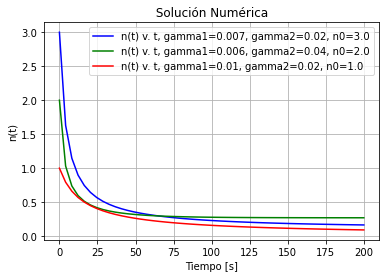
\includegraphics[scale=1]{figs/tdd_modelito1_sol_eq_diff_modificada.png}
    \caption{Se muestra un \textit{plot} de la solución numérica de la \eqref{eq:dif_model1} obtenida mediante la función odeint del paquete scipy del lenguaje Python para distintos parámetros de $\gamma_1,\gamma_2$ y $n_0$. Notamos que las soluciones tienen asíntotas horizontales cerca de cero pero distintas a cero.}
    \label{fig:tdd_modelito1_sol_eq_diff_odeint_multiples}
\end{figure}

En la figura \ref{fig:tdd_modelito1_sol_eq_diff_odeint_multiples} se muestran distintos plots de $n$ $vs$. $t$ para distintas condiciones iniciales de $\gamma_1, \gamma_2$ y número inicial de partículas $n_0$. Como se puede apreciar, vemos que el sistema termaliza, volviendo a su estado de equilibrio.

Resulta entonces que la dinámica de Lindblad para el hamiltoniano \eqref{model1_hamiltonian} resulta en una termalización a un estado con un número de ocupación fijo independientemente de la identidad del estado inicial del sistema.


\begin{Omitir}
Adicionalmente, el teorema de dilatación \cite{Stinespring,KasparovabtSt.} establece que toda evolución unitaria de un estado puede reescribirse en términos de una evolución unitaria conjunta entre el sistema de interés y otro sistema auxiliar, seguida de la traza parcial sobre el sistema auxiliar. Usando estos dos principios, el problema de modelado del sistema se reduce a aplicar correcciones a la ecuación de Schrödinger que sean capaz de reproducir el comportamiento del sistema.
\end{Omitir}
\begin{Omitir}
{\color{blue} Hasta aquí, no hablamos del entorno. Lo que habría que decir es algo así como que un sistema es \emph{cerrado} si su evolución depende de sus grados de libertad internos en forma determinista, o en otras palabras, que no interactúa con grados de libertad externos al sistema. 
Por otro lado, un sistema abierto es un sistema que no cumple con esta propiedad.  
En un sistema cerrado, la simetría ante traslaciones en el tiempo implica la evolución del estado está definida por la llamada Ecuación de Sch\"odinger\cite{HeinzPetruccione,Sch35}. En un sistema abierto, por otro lado, los grados de libertad se acoplan a grados de libertad no incluídos en la descripción (el entorno). El resultado de dicho acoplamiento es la introducción de efectos no deterministas en la evolución. Si podemos asumir que a pesar de no ser determinista, la evolución es continua, es posible modelarla en términos de la llamada ecuación de Lindblad\cite{HeinzPetruccione}\cite{Lindblad1976}.  }
\end{Omitir}



 

\begin{Omitir}
Corresponde ahora distinguir entre los sistemas físicos \textbf{cerrado} y \textbf{abierto}. Un sistema físico cerrado está completamente aislado de su exterior, mientras que un sistema físico abierto tiene interacciones con su entorno. Enunciamos, entonces, el siguiente postulado referente a la primera clase de estados (la discusión sobre sistemas físicos abiertos se hará en la siguientes secciones) 
\end{Omitir}




\begin{Omitir}

La definición anterior de un proceso de Markov no es inmediatamente útil para describir un proceso cuántico. En la mecánica cuántica es posible definir una distribución de probabilidad conjunta, la cual en general no cumplirá con las condiciones de Kolmogorov. Luego, las distribuciones de probabilidad conjuntas dadas en no se corresponderán a la jerarquía clásica de distribuciones de probabilidad conjuntas.

A tal fin, consideremos un observable de un sistema abierto cuántico $\mathbf{
X}$ a tiempos $t_n \geq t_{n-1} \geq \ldots \geq t_1 \geq 0$, el cual admite una descomposición espectral $\mathbf{X} = \sum_{x}x \ket{\phi_x}\bra{\phi_x}$. Luego, al evolucionar el estado del sistema, usando la regla de Born y mediante el postulado \ref{Post time evolution} tendremos una distribución de probabilidad conjunta

\begin{equation}
    P_n(x_n,t_n; x_{n-1},t_{n-1}; \ldots; x_{1},t_{1}) = \tr \{M_{x_n} \mathcal{U}_{t_n - t_{n-1}} \ldots M_{x_1} \mathcal{U}_{t_1} \rho(0)  \}
    \label{jpf-qm}
\end{equation}

la cual devuelve la probabilidad de medir una secuencia de resultados $x_n, x_{n-1},\ldots,x_1$
a tiempos $t_n, t_{n-1},\ldots,t_1$. Efectivamente, en mecánica cuántica es posible definir una distribución de probabilidad conjunta, la cual en general no cumplirá con las condiciones de Kolmogorov. Luego, las distribuciones de probabilidad conjuntas dadas en \eqref{jpf-qm} no se corresponden a la jerarquía clásica de distribuciones de probabilidad conjuntas. 
\end{Omitir}



\begin{Omitir}
\st{En muchos casos, es posible} capturar cualitativamente el comportamiento dinámico de algunos parámetros del sistema en estudio en forma analítica  o bien mediante el cálculo exacto o bien mediante la introducción de aproximaciones más o menos agresivas. Sin embargo, en muchos casos esto no es posible siendo necesario introducir herramientas informáticas para ganar conocimiento sobre el sistema y obtener predicciones más precisas. 
\st{Si se desea realizar una simulaci\'on num\'erica de un sistema cu\'antico solo se dispondr\'a de una cantidad finita de memoria para realizar los c\'alculos pertinentes, resultando no trivial el plasmado de las condiciones y propiedades del sistema a las rutinas y protocolos num\'ericos a implementar. Por ejemplo, si deseamos estudiar num\'ericamente un sistema bos\'onico con un espacio de Hilbert infinito-dimensional será necesario introducir un \textbf{procedimiento de truncamiento} para poder realizar los c\'alculos debido a esta escasez de recursos inform\'aticos. }


%\subsubsection{Procedimiento de truncamiento}

Existen múltiples procedimientos de truncamiento de un sistema, los dos relevantes a este trabajo son:

\begin{itemize}
    \item Truncar la base de operadores, procedimiento en el cual, \textit{a manu militari} se considera una base finita de solo algunos operadores y se elimina al resto.
    \item Truncar el espacio de Hilbert, procedimiento en el cual se limita un espacio de Hilbert infinto-dimensional a uno de dimensión finita $n$, siendo este $n$-ésimo nivel el \textit{cut-off}.
\end{itemize}

Cómo buscamos hacer simulaciones de dinámicas de sistemas bosónicos que tengan hasta correlaciones de dos cuerpos, en dichos casos hemos de implementar ambos procedimientos de truncamiento. Primero, hemos de truncar la base de operadores bosónicos incluyendo únicamente hasta operadores de dos cuerpos. Es decir consideraremos una base de operadores bosónicos $\{{\bf a}^{\dagger}{\bf a}, {\bf a}, {\bf a}^{\dagger},\mathds{1}\}$ con una normalización de forma tal que se cumpla el álgebra de operadores bosónicos. Para calcular esta renormalización de los operadores, hemos de truncar el espacio de Hilbert bosónico sobre el cual actuarán los operadores anteriores limitándolo al $n$-ésimo nivel. Luego, podremos ortonormalizar la base anterior siguiendo el teorema de Gram-Schmidt obteniendo que la nueva base de operadores será $\{{\bf a}^{\dagger}{\bf a}-\frac{n+1}{2}\mathds{1}, \frac{{\bf a}}{\sqrt{\frac{n(n+1)}{2}}}, \frac{{\bf a}^{\dagger}}{\sqrt{\frac{n(n+1)}{2}}}, \frac{\mathds{1}}{\sqrt{n}}\}$.
\end{Omitir}